\documentclass{bmvc2k}
\usepackage{ctex}  				 %支持中文
%% Enter your paper number here for the review copy
%\bmvcreviewcopy{??}

\title{节点分析社区挖掘等机器学习任务\\ ——基于学术文献网络}

% Enter the paper's authors in order
% \addauthor{Name}{email/homepage}{INSTITUTION_CODE}
%\addauthor{Susan Student}{http://www.vision.inst.ac.uk/~ss}{1}
%\addauthor{Petra Prof}{http://www.vision.inst.ac.uk/~pp}{1}
%\addauthor{Colin Collaborator}{colin@collaborators.com}{2}

\addauthor{黄之豪 }{20110980005@fudan.edu.cn}{1}
\addauthor{周笑宇}{20210980066@fudan.edu.cn}{1}
\addauthor{王嘉炜}{20210840012@fudan.edu.cn}{2}


% Enter the institutions
% \addinstitution{Name\\Address}
\addinstitution{
大数据学院
}
\addinstitution{
数学科学学院
}

\runninghead{社交网络分析PJ}{第34小组}

% Any macro definitions you would like to include
% These are not defined in the style file, because they don't begin
% with \bmva, so they might conflict with the user's own macros.
% The \bmvaOneDot macro adds a full stop unless there is one in the
% text already.
\def\eg{\emph{e.g}\bmvaOneDot}
\def\Eg{\emph{E.g}\bmvaOneDot}
\def\etal{\emph{et al}\bmvaOneDot}

%-------------------------------------------------------------------------
% Document starts here
\begin{document}

\maketitle

\begin{abstract}
本次社交网络分析作业中,我们小组主要完成了如下工作:1.通过选取关键词及爬虫,获取了金融、CS领域10个细分关键词的总共229万条文献数据;2.计算网络统计属性;3.进行网络节点分析;4.基于异构文献网络学术合作预测;5.通用预训练文献网络Embedding;6.文献Abstract相似性分析;7.网页、作图等项目可视化。
\end{abstract}

%-------------------------------------------------------------------------
\section{Data}
%\label{sec:intro}
首先,小组成为根据专业特点和课程特点(如:social network analysis)确定了金融和CS两大主题和两大主题下10个细分主题:financial pricing, financial risk management, financial risk measurement, behavior finance, corporate finance, fintech, financial supervision, deep learning, machine learning, social network analysis。

将这些关键词作为web of science搜索的keywords进行文章爬取,去除没有doi的文章,总共获得种子文章263,698篇。进一步抓取种子文章的参考文献,最终总共获得了2,298,732篇不重复的文献数据。考虑到mongo在修改数据、数据库结构方面便捷性优势较大,使用mongo数据库。

字段及相关说明如下表所示(网盘中有"deep learning"为关键词的详细数据):

\begin{table}
	\begin{center}
%		\resizebox{\textwidth}{15mm}{
		\begin{tabular}{| l |l| l |p{3cm} |} 
%			\begin{tabular}{cccc} 
			\hline 
			字段名 & 说明  & 字段名 & 说明 \\ 
			\hline\hline
			\_id & doi & publication\_type  & 文献类型(Journal,book等) \\ 
			\hline 
			authors & 作者 & authors\_full\_name & 作者全名 \\ 
			\hline 
			title & 题目 & num\_id & 自己给予的unique编号  \\ 
			\hline 
			pub\_year & 发表年份 & research\_areas & 作者研究领域 \\ 
			\hline 
			abstract & 摘要  & wos\_id & Web Of Science文章编码 \\ 
			\hline 
			issn & issn编号 & big\_topic & Finance / CS \\ 
			\hline 
			journal & 发表期刊 & topic\_field & 10大细分领域中的一个或多个 \\ 
			\hline 
			keywords & 关键词 & author\_address & 作者工作地址   \\ 
			\hline 
			issue & 期刊issue & cited\_number & 其他文章引用该文章数 \\ 
			\hline 
			crawl\_time & 爬取时间 & cite\_references\_number & 引用其他文章数 \\ 
			\hline 
			vol & 期刊vol & category & WOS领域分类 \\ 
			\hline 
			lang & 语言 & keywords\_plus & 更多关键词   \\ 
			\hline 
			publisher & 出版商 & reference & 文章引用文章的doi list \\
			\hline 
			pub\_date & 发表日期 & &    \\
			\hline 
		\end{tabular} 
	\end{center}
	\caption{数据库字段及说明}
\end{table}



%-------------------------------------------------------------------------
\section{网络的统计属性}
在网络的统计属性上,我们抽取主题为Deep Learning 领域的文章构建作者合作网络,计算了平均度,平均聚类系数等属性,如表所示。同时,作出作者合作网络(图1左)及文献引用网络(图1右)中的度分布图,可明显看出度是服从幂律分布的。\\
\indent 进一步,我们采用Louvain算法对作者合作网络进行了社区划分,该算法目标是最大化模块度,能够发现层次化的社区结构。可视化展现前几个社区,可见整个作者的合作网络是比较离散的,几位作者之间往往会构成学术团体,团体内部合作紧密,外部合作较少。
\begin{table}[h]
\begin{center}
\begin{tabular}{|c|c| } 
	\hline 
	平均度 &5.003\\ 
	\hline
	平均聚类系数& 0.994\\ 
	\hline 
	平均路径长度 & 1.16 \\ 
	\hline 
	最大联通子图直径 &3 \\ 
	\hline 	
\end{tabular} 
\end{center}
\caption{作者合作网络属性}
\end{table}

\begin{figure}[htbp]
\centering
\begin{minipage}[t]{0.48\textwidth}
\centering
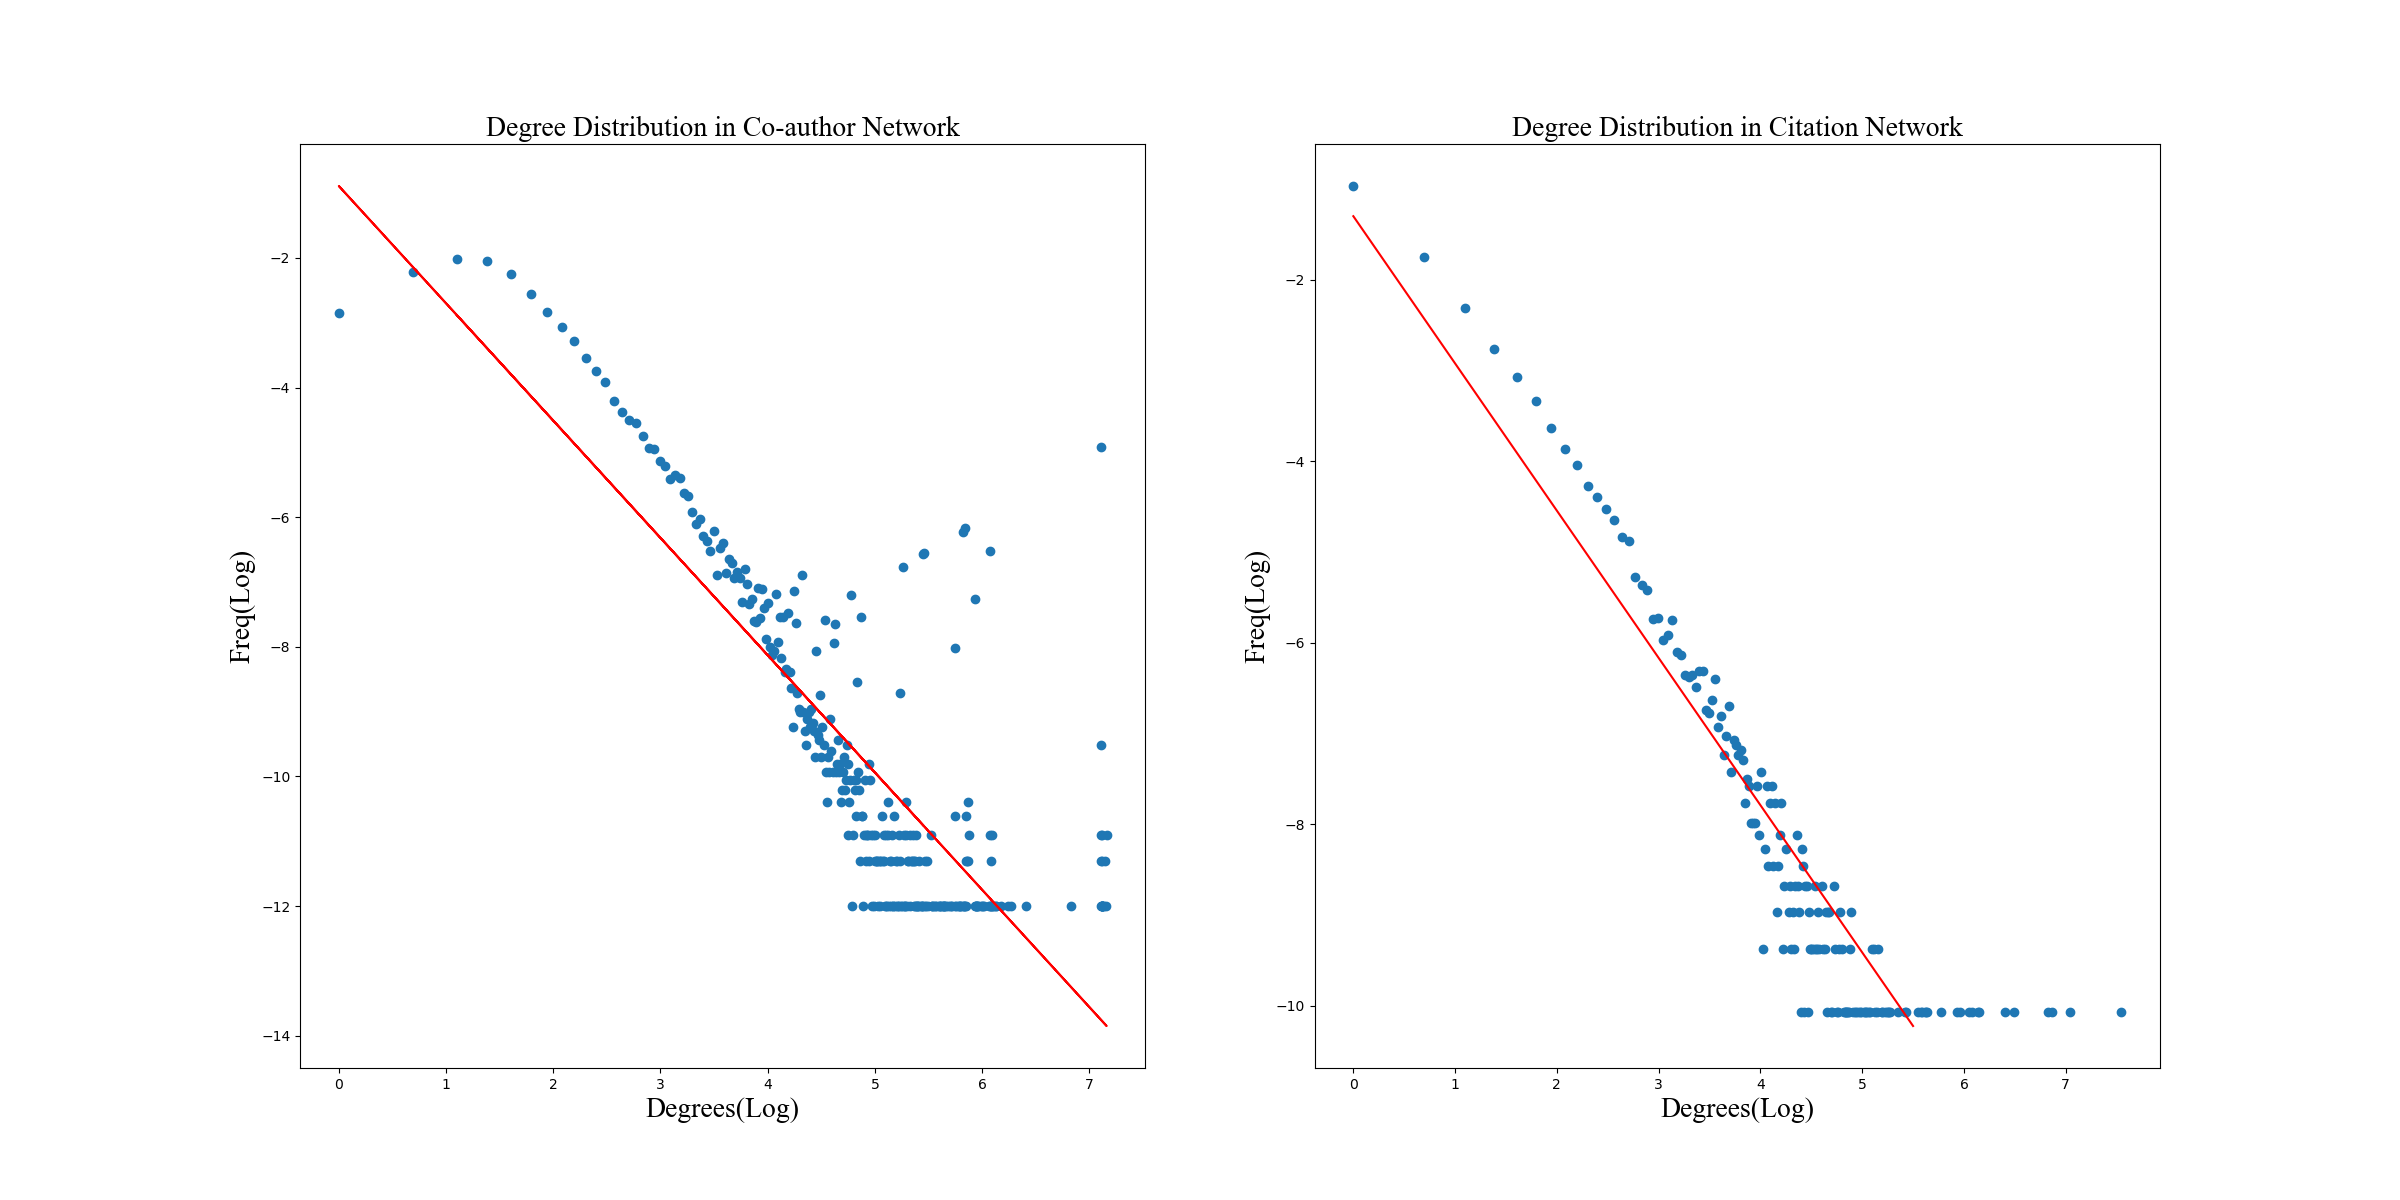
\includegraphics[width=7cm]{images/degee_dis.png}
\caption{度分布}
\end{minipage}
\begin{minipage}[t]{0.48\textwidth}
\centering
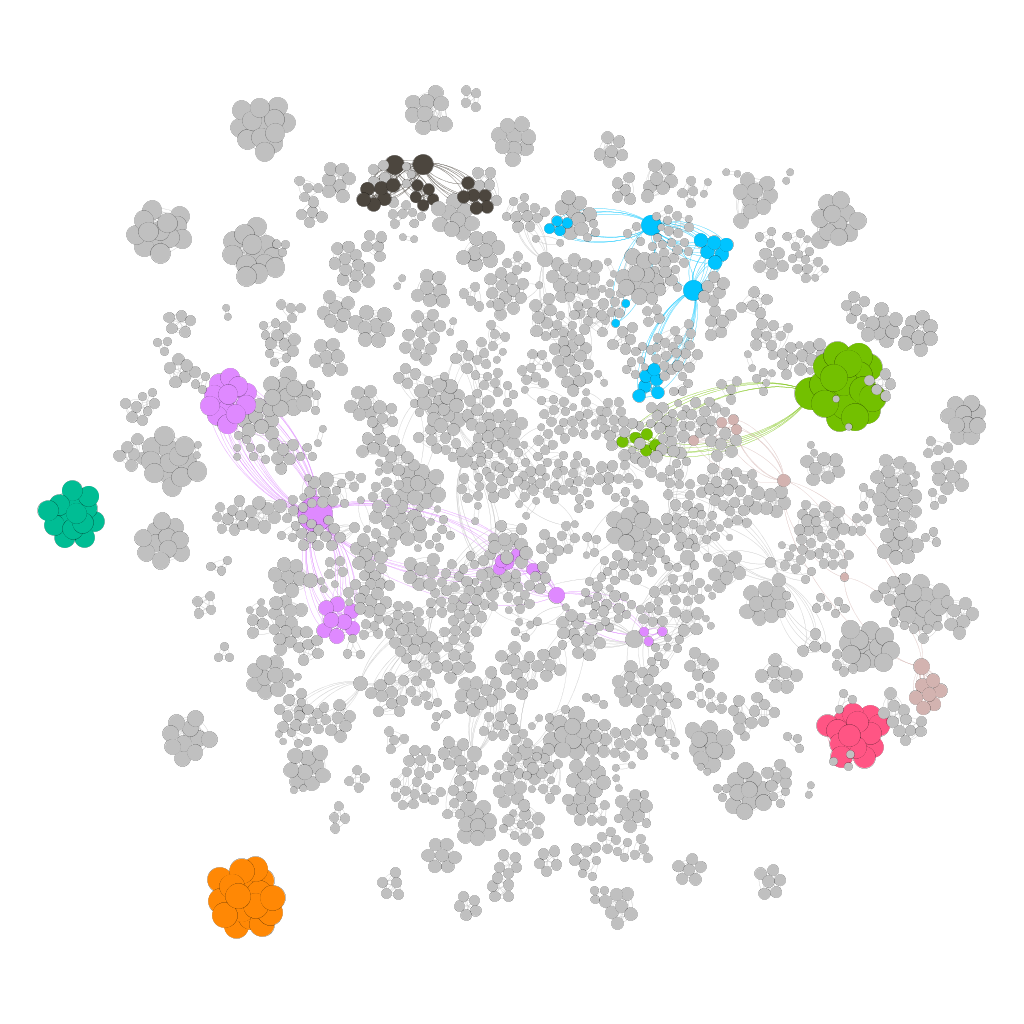
\includegraphics[width=3.5cm]{images/community.png}
\caption{社区可视化}
\end{minipage}
\end{figure}


%\begin{figure}
%\begin{tabular}{ccc}
%\bmvaHangBox{\fbox{\parbox{2.7cm}{~\\[2.8mm]
%\rule{0pt}{1ex}\hspace{2.24mm}\includegraphics[width=2.33cm]{images/eg1_largeprint.png}\\[-0.1pt]}}}&
%\bmvaHangBox{\fbox{\includegraphics[width=2.8cm]{images/eg1_largeprint.png}}}&
%\bmvaHangBox{\fbox{\includegraphics[width=5.6cm]{images/eg1_2up.png}}}\\
%(a)&(b)&(c)
%\end{tabular}
%\caption{It is often a good idea for the first figure to attempt to
%encapsulate the article, complementing the abstract.  This figure illustrates
%the various print and on-screen layouts for which this paper format has
%been optimized: (a) traditional BMVC print format; (b) on-screen
%single-column format, or large-print paper; (c) full-screen two column, or
%2-up printing. }
%\label{fig:teaser}
%\end{figure}

\section{网络节点分析}
\subsection{针对论文节点}
在论文引用网络中,包含节点(论文)和有向边(引用,由引用指向被引用)。这些图的性质能够帮助我们更好的度量节点的中心性,从而找出影响力最大的论文。
在项目中我们使用的计算中心性的算法包括:
\begin{enumerate}
\item 特征向量中心性

通过结合无向图中的邻居节点,或者有向图中的输入邻居节点的重要性来概括中心度。
\item PageRank

将中心性除以节点的外连接(出度)的数目,使得每个邻居节点获得源结点中心性的一部分。
\item 接近中心性

若一个节点越趋于中心,则其能够更快速到达其它节点,即它与其他节点之间有最小平均最短距离。
\end{enumerate}
\subsection {针对作者节点}
通过上述方式我们计算出论文的影响力(中心性),记为$IF(u_i)$。我们希望通过论文的影响力来衡量作者影响力,我们设计了如下算法:
\begin{enumerate}
\item 将每篇论文的影响力$IF(u_i)$均分给该论文的所有作者,每位作者获得的影响力为$\frac{IF(u_i)}{n(u_i)}$,$n(u_i)$为论文$u_i$的作者数。
\item 将作者$v_i$从其发表的论文中所获得的影响力求和,$\sum_{v_i}\frac{IF(u_i)}{n(u_i)} $,作为$v_i$的初始影响力。
\item 根据作者合作网络,利用改进的PageRank算法计算,迭代过程如下:
\[ C_p(v_i) = \alpha\sum_{j=1}^{n}A_{i,j}\frac{C_p(v_j)}{d_j^{out}}+\beta(v_i) \]
\[ A_{i,j} = \ln(k_{i,j}) + 1 \]
\[ \beta(v_i) = \sum_{v_i}\frac{IF(u_i)}{n(u_i)} \]
其中$k_{i,j}$表示两个作者之间的合作次数,$u_i \in \{$作者$v_i$写过的论文$\}$。
\item 直到$ C_p(v_i)$收敛,迭代终止,得到所有作者最终的中心性值(影响力)。
\end{enumerate}
为了衡量我们算法的效果,根据我们计算的中心性值对作者进行排序,将Google Scholar中作者的总被引用次数的排名结果作为参照集,取前十五位学者,结果如下,两种排序的Spearman系数为0.86。
\begin{table}[h]
\begin{center}
\begin{tabular}{|c|c|c|c|c|c|c|c|c|c|c|c| } 
	\hline 
	Pr值排序 &1 &2 &3 &4 &5 &6  &7 &8 &9 &10 & ... \\ 
	\hline
	总被引用数& 1 &2 &4 &3 &8 &9 &7 &6 &5 &14 &...\\ 
	\hline 
\end{tabular} 
\end{center}
\caption{两种排名比较}
\end{table}

\section{ 学术合作预测}
针对学术合作预测问题,传统的同构网络只包含单一类型的节点,这种网络结构包含的拓扑信息有限,往往难以揭露深层次的规律。因此,为了充分利用已知信息来对未来合作进行预测,我们考虑异构学术网络。在异构网络中不仅包含作者节点,还包含论文节点、主题节点、期刊节点以及连接它们的边,节点之间的关系也更加复杂。受到2011年发表于ASONAM上论文的启发,异构网络中不同节点间复杂的关系衍生出了元路径的概念,针对每一种元路径,都可以计算该路径的异构拓扑特征,如Path Count、Symmetric Random Walk
等,最后将这些特征输入到二分类模型中,来对作者合作与否做出预测。

在实验过程中,我们选取了“作者-论文-共同合作者-论文-作者”,“作者-论文-共同引用论文-论文-作者”,“作者-论文-期刊-论文-作者”这三类元路径,在下文中我们简记为“A-P-A-P-A”,“A-P$\to P\gets$P-A”,“A-P-V-P-A”。我们计算这三类关系的Symmetric Random Walk(SRW)值作为特征,计算方式如下:
\[
\begin{split} SRW_R(a_i,a_j) &= RW_R(a_i,a_j) + RW_{R^{-1}}(a_j,a_i) \\
&= \frac{PC_R(a_i,a_j)}{PC_R(a_i,\cdot)} + \frac{PC_{R^{-1}}(a_j,a_i)}{PC_{R^{-1}}(\cdot,a_j)}
\end{split}
\]
其中$PC_R(a_i,\cdot)$表示以一定规则的从$a_i$出发的所有路径之和,$PC_R(\cdot,a_j)$表示以一定规则的以$a_j$为结尾的所有路径之和。

采取逻辑回归模型进行分类,首先将数据集按照时间段分成三部分:$T_0$=[2003年,2008年],$T_1$=[2009年,2014年],$T_2$=[2015年,2018年],将$T_0$和$T_1$的合作数据记录下来作为训练集,将$T_1$和$T_2$的合作数据记录下来作为测试集。训练模型中,给出特征的显著性如下:
\[
\begin{tabular}{|c|c|c|}
\hline
Meta Path + Measure & Coefficient & P-value \\ \hline
A-P-A-P-A + SRW  & 0.9366 & 0.016 \\
A-P$\to P\gets$P-A + SRW & 0.5285 & 0.060 \\
A-P-V-P-A + SRW & 0.4482 & 0.142 \\
\hline
\end{tabular}
\]

由此可见,作者之间发生学术合作的概率与他们有共同合作者高度相关,相关性次之的是共同引用同一篇论文,最后是在同一种期刊发表过论文。这也与实际情况相符合:一般而言,若两人有共同合作者,则他们无论是在学术交流还是在现实生活中接触的概率都要远大于另两种情况,因此这种特征在分类模型中表现极为显著,而引用同一篇论文则暗含两者有相同或相近的研究方向,这比只是在同一领域的以期刊为桥梁的关系无疑要更为密切。

最后,我们根据训练的逻辑回归模型对未来学术合作进行预测,输出的混淆矩阵如下图所示:
\begin{figure}[h]
\centering
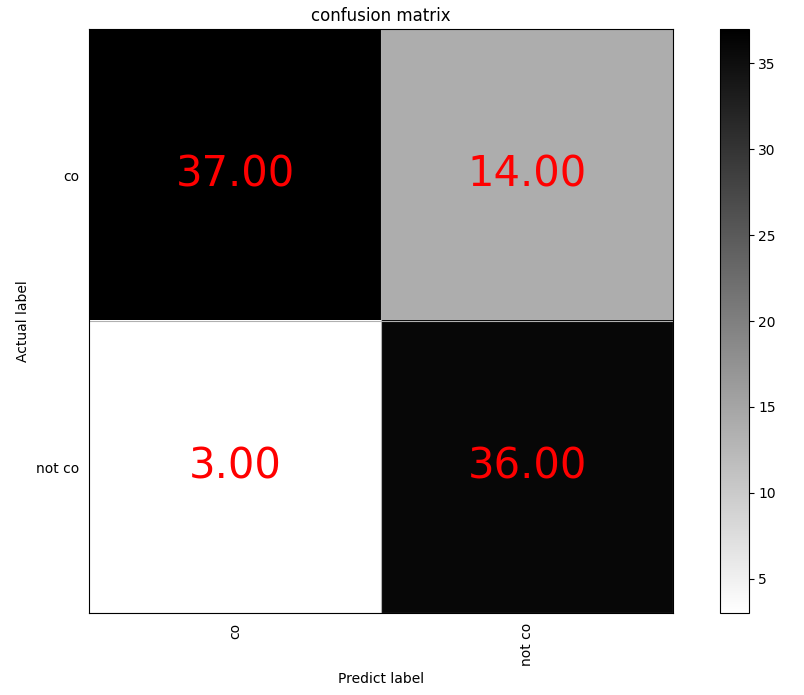
\includegraphics[width=2in]{images/confussion.png}
\caption{预测结果}
\end{figure}

可以看到,我们的模型对于未来不会发生合作的情况预测的非常准确,对于未来会发生合作的学者预测也有较高的准确率。



\section{Metapath2vec}
%\label{sec:intro}
Metapath2vec是Yuxiao Dong等\cite{10.1145/3097983.3098036}于2017年提出的一种用于异构信息网络(Heterogeneous Information Network, HIN)的顶点嵌入方法。metapath2vec使用基于meta-path的random walks来构建每个顶点的异构邻域,然后用Skip-Gram模型来完成顶点的嵌入。在metapath2vec的基础上,作者还提出了metapath2vec++来同时实现异构网络中的结构和语义关联的建模。

本文的主要贡献在于:先前针对同构网络提出的embedding方法无法保留异构网络中的"节点上下文(word-context)"信息,使用metapath方法最大化保留给定异构网络的结构和语义。开发了一种基于异构负采样的,称为metapath2vec++的方法,该方法可以准确而有效地预测节点的异构邻域。

\subsection{The Metapath2vec Framework}
Metapath2vec模型思想、代码部分很大程度都借鉴了Mikolov等(2013) word2vec\cite{10.5555/2999792.2999959}的思想。以下主要根据Metapath2vec模型的几处创新点进行模型框架概述:

该文章最大贡献在于根据异构网络特性,提出基于预先指定的元路径(meta-path)来进行随机游走,预先构造路径能够保持"节点上下文"的概念。 meta-path scheme  定义
$\mathcal{P}: V_{1} \stackrel{R_{1}}{\longrightarrow} V_{2} \stackrel{R_{2}}{\longrightarrow} \cdots V_{t} \stackrel{R_{t}}{\longrightarrow} V_{t+1} \cdots \stackrel{R_{l-1}}{\longrightarrow} V_{l}$ ,其中,$R=R_{1} \circ R_{2} \circ \cdots \circ R_{l-1}$ 代表 $V_{1}$ 到 $V_{l}$ 这些节点间的关系。如图所示,例如"APA"(作者-文章-作者)就是一条元路径(工程上来说论文源代码和本次PJ都使用"期刊-作者-期刊"的元路径)

\begin{figure}[htb]
	\begin{center}
		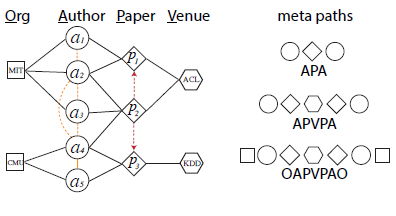
\includegraphics{images/metapath.png}
	\end{center}
	%\begin{tabular}{ccc}
	%	
	%\bmvaHangBox{\fbox{\parbox{2.7cm}{~\\[2.8mm]
	%\rule{0pt}{1ex}\hspace{2.24mm}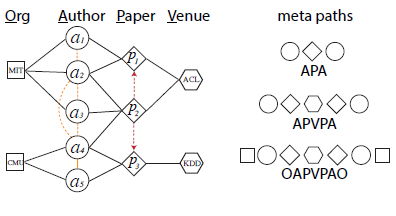
\includegraphics[width=2.33cm]{images/metapath.png}\\[-0.1pt]}}}&
	%\bmvaHangBox{\fbox{\includegraphics[width=2.8cm]{images/eg1_largeprint.png}}}&
	%\bmvaHangBox{\fbox{\includegraphics[width=5.6cm]{images/eg1_2up.png}}}\\
	%(a)&(b)&(c)
	%\end{tabular}
	%\caption{It is often a good idea for the first figure to attempt to
	%encapsulate the article, complementing the abstract.  This figure illustrates
	%the various print and on-screen layouts for which this paper format has
	%been optimized: (a) traditional BMVC print format; (b) on-screen
	%single-column format, or large-print paper; (c) full-screen two column, or
	%2-up printing. }
	\caption{文献 meta-path 示例}
	\label{fig:teaser}
\end{figure}

%\begin{figure*}
%\begin{center}
%\fbox{\rule{0pt}{2in} \rule{.9\linewidth}{0pt}}
%\end{center}
%   \caption{Example of a short caption, which should be centered.}
%\label{meta-path 示例}
%\end{figure*}

%第i步转移概率定义如下:
%$$
%p\left(v^{i+1} \mid v_{t}^{i}, \mathcal{P}\right)=\left\{\begin{array}{cl}
%\frac{1}{\left|N_{t+1}\left(v_{t}^{i}\right)\right|} & \left(v^{i+1}, v_{t}^{i}\right) \in E, \phi\left(v^{i+1}\right)=t+1 \\
%0 & \left(v^{i+1}, v_{t}^{i}\right) \in E, \phi\left(v^{i+1}\right) \neq t+1 \\
%0 & \left(v^{i+1}, v_{t}^{i}\right) \notin E
%\end{array}\right.
%$$
%
文章第二大贡献在于提出基于异构网络的负采样,即 metapath2vec++,具体地,通过具体到某个类型节点的邻居取代所有类型进行负采样。
%
%$$
%p\left(c_{t} \mid v ; \theta\right)=\frac{e^{X_{c_{t}} \cdot X_{v}}}{\sum u_{t} \in V_{t} e^{X_{u_{t}} \cdot X_{v}}}
%$$
%
%$$
%O(\mathrm{X})=\log \sigma\left(X_{c_{t}} \cdot X_{v}\right)+\sum_{m=1}^{M} \mathrm{E}_{u_{t}^{m} \sim P_{t}\left(u_{t}\right)}\left[\log \sigma\left(-X_{u_{t}^{m}} \cdot X_{v}\right)\right]
%$$

生成随机游走: 1000次随机游走, 每次10步。Embedding参数: 128维, skip-gram window 7, negative sampling 5。实验效果:通过使用metapath2vec训练Embedding后,通过相似度匹配,找到与某个期刊最相近的期刊,QUANTITATIVE FINANCE和MACHINE LEARNING为例,得到与之最为相似的期刊如下:

\begin{table}
	\begin{center}
		\resizebox{\textwidth}{15mm}{
		\begin{tabular}{| l |l|l|} 
			\hline 
			Rank &QUANTITATIVE FINANCE &MACHINE LEARNING  \\ 
			\hline
			1& Complexity,Metastability and Nonextensivity &2018IEEE/ACM40TH INTERNATIONAL CONFERENCE ON SOFTWARE ENGINEERING \\ 
			\hline
			2& MARKET MICROSTRUCTURE AND LIQUIDITY &ECAI2010-19TH EUROPEAN CONFERENCE ON ARTIFICIAL INTELLIGENCE \\
			\hline
			3& MATHEMATICAL CONTROL THEORY AND FINANCE &PROCEEDINGS OF THE 12TH INTERNATIONAL CONFERENCE ON WEB INFORMATION SYSTEMS AND TECHNOLOGIES \\
			\hline
			4& NUMERICAL COMPUTATIONS:THEORY AND ALGORITHMS &MATHEMATICAL PROGRAMMING COMPUTATION \\
			\hline
			5& FROM STOCHASTIC CALCULUS TO MATHEMATICAL FINANCE &ARTIFICIAL INTELLIGENCE IN MEDICINE \\
			\hline 
		\end{tabular} }
	\end{center}
	\caption{训练的Embedding效果展示}
\end{table}

根据先验知识,量化金融确实与数值计算、数学控制、随机分析等有着密不可分的关系,结合网盘中的Embedding降维成三维之后展示效果,可以看出,Embedding质量较好。

\section{摘要相似度}
这里选取了Zhelezniak等(2019)\cite{2019arXiv190507790Z}的baseline文本相似度分析方法,通过word2vec, Glove, ELMo三种词向量模型和avg\_cosine, pearson, spearman,
kendall, apsyn, apsynp六个向量相似度度量指标来计算摘要的相似度,部分结果如可视化网页所示。
%\begin{table}
%	\begin{center}
%%		\resizebox{\textwidth}{15mm}{
%			\begin{tabular}{| c |c|} 
%				\hline 
%				Abstract1 &Abstract2  \\ 
%				\hline
%				Company disclosures greatly aid in the process of financial decision-making; therefore, they are consulted by financial investors and automated traders before exercising ownership in stocks. While humans are usually able to correctly interpret the content, the same is rarely true of computerized decision support systems, which struggle with the complexity and ambiguity of natural language. A possible remedy is represented by deep learning, which overcomes several shortcomings of traditional methods of text mining. For instance, recurrent neural networks, such as long short-term memories, employ hierarchical structures, together with a large number of hidden layers, to automatically extract features from ordered sequences of words and capture highly non-linear relationships such as context-dependent meanings. However, deep learning has only recently started to receive traction, possibly because its performance is largely untested. Hence, this paper studies the use of deep neural networks for financial decision support. We additionally experiment with transfer learning, in which we pre-train the network on a different corpus with a length of 139.1 million words. Our results reveal a higher directional accuracy as compared to traditional machine learning when predicting stock price movements in response to financial disclosures. Our work thereby helps to highlight the business value of deep learning and provides recommendations to practitioners and executives. (C) 2017 Elsevier B.V. All rights reserved."  &Predicting the final closing price of a stock is a challenging task and even modest improvements in predictive outcome can be very profitable. Many computer-aided techniques based on either machine learning or statistical models have been adopted to estimate price changes in the stock market. One of the major challenges with traditional machine learning models is the feature extraction process. Indeed, extracting relevant features from data and identifying hidden nonlinear relationships without relying on econometric assumptions and human expertise is extremely complex and makes deep learning particularly attractive. In this paper, we propose a deep neural network-based approach to predict if the stock price will increase by 25\% for the following year, same quarter or not. We also compare our deep learning method against 'shallow' approaches, random forest and gradient boosted machines. To test the proposed methods, KIS-VALUE database consisting of the Korea Composite Stock Price Index (KOSPI) of companies for the period 2007 to 2015 was considered. All the methods yielded satisfactory performance, namely, deep neural network achieved an AUC of 0.806. 'Shallow' approaches, random forest and gradient boosted machines have been used for comparisons. \\
%				
%				\hline 
%		\end{tabular} 
%	\end{center}
%	\caption{训练的Embedding效果展示}
%\end{table}



\section{小组分工}
\noindent 周笑宇:负责整体模型思路的设计,网络的统计属性和社区划分的编程实现,PPT以及讲稿制作。\\
\noindent 黄之豪:负责爬虫,Metapath2Vec以及摘要相似度的编程实现以及节点三维可视化,项目的网页可视化。\\
\noindent 王嘉炜:负责节点分析、作者学术合作预测的编程实现。



%For this citation style, keep multiple citations in numerical (not
%chronological) order, so prefer


%-------------------------------------------------------------------------
%\subsection{Footnotes}




%\begin{figure*}
%\begin{center}
%\fbox{\rule{0pt}{2in} \rule{.9\linewidth}{0pt}}
%\end{center}
%   \caption{Example of a short caption, which should be centered.}
%\label{fig:short}
%\end{figure*}

%-------------------------------------------------------------------------







%------------------------------------------------------------------------


\bibliography{egbib}
\end{document}
